\renewcommand{\theequation}{\theenumi}
\begin{enumerate}[label=\arabic*.,ref=\thesubsection.\theenumi]
\item Find the distance of the point $\myvec{4\\2\sqrt{3}}$ from the line 
\begin{equation}
\myvec{\cos 60\degree &  \sin 60\degree}\vec{x} = 6
\end{equation}
\numberwithin{equation}{enumi}
\item Find the distance of the point $\myvec{2\\3}$ from each of the straight lines 
\begin{align}
\myvec{5&12}\vec{x}-20&=0
\\
 \myvec{4&-3}\vec{x}+11&=0
\\
 \myvec{3 & 4}\vec{x}-28&=0.
\end{align}
\renewcommand{\theequation}{\theenumi}
\item Find the distance of the pont $\myvec{3\\-1}$ from the line joining the points $\myvec{2\\-3}$, $\myvec{4\\1}$.
\item Are the points $\myvec{-2\\3}$, $\myvec{-2\\4}$ on the same or on opposite sides of the line
\begin{align}
\myvec{4 &5} \vec{x}= 10?
\end{align}
\numberwithin{equation}{enumi}
\item Find the equations of the bisectors of the angles between the lines
\begin{align}
\myvec{-4 &2}\vec{x}&=-9
\\
\myvec{-1 & 2}\vec{x}&= 4
\end{align}
and state which equation refers to the angle which contains the origin.
\item Prove that the bisector of one of the angles between the lines
\begin{align}
\myvec{5&1}\vec{x}-7 &= 0
\\
\myvec{1 & -5}\vec{x}+7 &= 0
\end{align}
passes through the origin.  What is the equation of the bisector of the other angle?
\renewcommand{\theequation}{\theenumi}
\item What is the condition that the point $\myvec{x\\y}$ may be at unit distance from the line
\begin{align}
\myvec{3 &-4}\vec{x}+10 = 0
\end{align}
Write down the equations of two straight lines parallel to the given line and at unit distances from it,
and state which of the two lies on the same side of the given line as the origin.
\item The sides $AB$, $BC$, $CA$ of a triangle have equations
\numberwithin{equation}{enumi}
\begin{align}
\myvec{4&-3} \vec{x}&= 12
\\
\myvec{ 3 &4} \vec{x}&= 24
\\
\myvec{0 & 1} \vec{x}&= 2.
\end{align}
Find the coordinates of the centres of the inscribed circle and of the escribed circle opposite to the vertex $\vec{A}$.
\item Prove that the point $\myvec{4\\4}$ lies outside the triangle whose sides are the lines
\begin{align}
\myvec{3&4} \vec{x}&= 24
\\
\myvec{ 5 & - 3} \vec{x}&= 15
\\
\myvec{0 &1} \vec{x}&= 0
\end{align}
\item Find the equation of the line joining the origin to the point of intersection of the lines
\begin{align}
\myvec{1&7}\vec{x} - 11 &= 0
\\
\myvec{-2 & 1} \vec{x}= 3
\end{align}
\item Find the equation of a line perpendicular to the line
\begin{align}
\myvec{3&5}\vec{x}+11 = 0
\end{align}
and passing through the intersection of the lines
\begin{align}
\myvec{5 & - 6} \vec{x}&= 1
\\
\myvec{ 3&2}\vec{x}+5 &= 0
\end{align}
\item Find the equation of a line through the intersection of the lines
\begin{align}
\myvec{2&5} \vec{x}&= 1
\\
\myvec{-4 & 1} \vec{x}&= 9
\end{align}
parallel to the line 
\begin{align}
\myvec{1 & 1} \vec{x}= 1
\end{align}
\renewcommand{\theequation}{\theenumi}
%
\item The vertices of a triangle are at the points
\begin{align}
\vec{A},
\vec{B},
\vec{C}
\end{align}
Find the equations of the medians and prove that they meet in a point.  What are the coordinates of their point of intersection?
\numberwithin{equation}{enumi}
\\
 $BE$ and $CF$ are medians of $\triangle ABC$ intersecting at $\vec{O}$ as shown in Fig. \ref{fig:median}. 
We first  show that
\begin{equation}
\frac{CO}{OF} = \frac{BO}{OE} = 2
\end{equation}
%
\begin{figure}[!hb]
\centering
\includegraphics[width=\columnwidth]{./figs/median.eps}
\caption{}
\label{fig:median}
\end{figure}
 Let
\begin{align}
\frac{CO}{OF} &= k_1
\\
\frac{BO}{OE} &= k_2
\end{align}
%
Using  \eqref{eq:ratio},
\begin{align}
\vec{E}&= \frac{\vec{A} + \vec{C}}{2}
\\
\vec{F}&= \frac{\vec{A} + \vec{B}}{2}
\end{align}
%
and
\begin{align}
\label{eq:o1}
\vec{O}&= \frac{k_1\vec{F} + \vec{C}}{k_1+1} = \frac{k_1\frac{\vec{A} + \vec{B}}{2} + \vec{C}}{k_1+1}
\\
\vec{O}&= \frac{k_2\vec{E} + \vec{B}}{k_2+1} = \frac{k_2\frac{\vec{A} + \vec{C}}{2} + \vec{B}}{k_2+1}
\label{eq:o2}
\end{align}
%
From \eqref{eq:o1} and \eqref{eq:o2},
\begin{align}
 \frac{k_1\frac{\vec{A} + \vec{B}}{2} + \vec{C}}{k_1+1} &= 
 \frac{k_2\frac{\vec{A} + \vec{C}}{2} + \vec{B}}{k_2+1}
\end{align}
\begin{multline}
\label{eq:lin_comb}
\implies \sbrak{\frac{k_1\brak{k_2+1}}{2}
-\frac{k_2\brak{k_1+1}}{2}}\vec{A} 
\\
+ 
\sbrak{\frac{k_1\brak{k_2+1}}{2}-\brak{k_1+1}}\vec{B} 
\\
+ \sbrak{\brak{k_2+1}-\frac{k_2\brak{k_1+1}}{2}}\vec{C} 
= 0
\end{multline}
resulting in $k_1 = k_2$,
\begin{align}
k_1^2-k_1-2  &= 0
\implies k_1 = k_2 = 2,
\end{align}
provided $\vec{A},\vec{B},\vec{C}$ are linearly independent. Thus, substituting $k_1=2$ in \eqref{eq:o2},
\begin{equation}
\vec{O} = \frac{\vec{A}+\vec{B}+\vec{C}}{3}
\end{equation}
%
If $\vec{A},\vec{B},\vec{C}$ are linearly dependent,
\begin{align}
\label{eq:lin_dep}
\vec{A} = \alpha \vec{B} + \beta \vec{C} 
\end{align}
%
Note that $\vec{B},\vec{C}$ are linearly independent.
Substituting \eqref{eq:lin_dep} in \eqref{eq:lin_comb},
\begin{multline}
%\label{eq:lin_comb}
 \sbrak{\frac{k_1\brak{k_2+1}}{2}
-\frac{k_2\brak{k_1+1}}{2}}\sbrak{\alpha \vec{B} + \beta \vec{C}  }
\\
+ 
\sbrak{\frac{k_1\brak{k_2+1}}{2}-\brak{k_1+1}}\vec{B} 
\\
+ \sbrak{\brak{k_2+1}-\frac{k_2\brak{k_1+1}}{2}}\vec{C} 
= 0
\end{multline}
\begin{align}
\implies
\begin{split}
\brak{k_1-k_2}\alpha + k_1k_2 - k_1-2 &=0
\\
\brak{k_1-k_2}\beta - k_1k_2 + k_2+2 &=0
\end{split}
\label{eq:median_contra}
\\
\implies \brak{k_1-k_2}\brak{\alpha +\beta - 1} = 0
\end{align}
If $\alpha+\beta = 1, \vec{A},\vec{B},\vec{C}$ are collinear according to \eqref{eq:ratio} resulting in a 
contradiction.  Hence, $k_1=k_2$, which, upon substitution in \eqref{eq:median_contra}, yields
\begin{equation}
k_1^2 - k_1-2 = 0 \implies k_1 = 2.
\end{equation}

\item For what multiples $k, l, m$ is the equation
\begin{align}
k\cbrak{\myvec{2&3}\vec{x}-13}+l\cbrak{\myvec{5& -y}\vec{x}-7} 
\nonumber \\ 
+ m\cbrak{\myvec{1 &-4}\vec{x}+10} = 0
\end{align}
an identity?  In what point do the lines given by equating the three terms to zero concur?
\item Find the equations of the diagonals of the parallelogram
\begin{align}
\myvec{2&-1} \vec{x}+7&= 0
\\
\myvec{ 2 &-1}\vec{x}-5 &= 0,
\\
\myvec{ 3 &2}\vec{x}-5 &= 0
\\
\myvec{ 3 &2}\vec{x}+4&=0 
\end{align}
\renewcommand{\theequation}{\theenumi}
\item The vertices of a triangle are at the points
\begin{align}
\myvec{2\\3}, \myvec{4\\-3}, \myvec{-2\\1}
\end{align}
Find the equations of the perpendiculars to the sides through their middle points.
\numberwithin{equation}{enumi}
\item Work the same problem when the vertices of the triangle are at the points
\begin{align}
\vec{A},
\vec{B},
\vec{C}
\end{align}
and show that the perpendiculars meet in a point.
\\%
\solution In Fig. \ref{fig:alt}, $BE \perp AC, CF \perp AB$.  We need to show that $AD \perp BC$.
\begin{figure}[!hb]
\centering
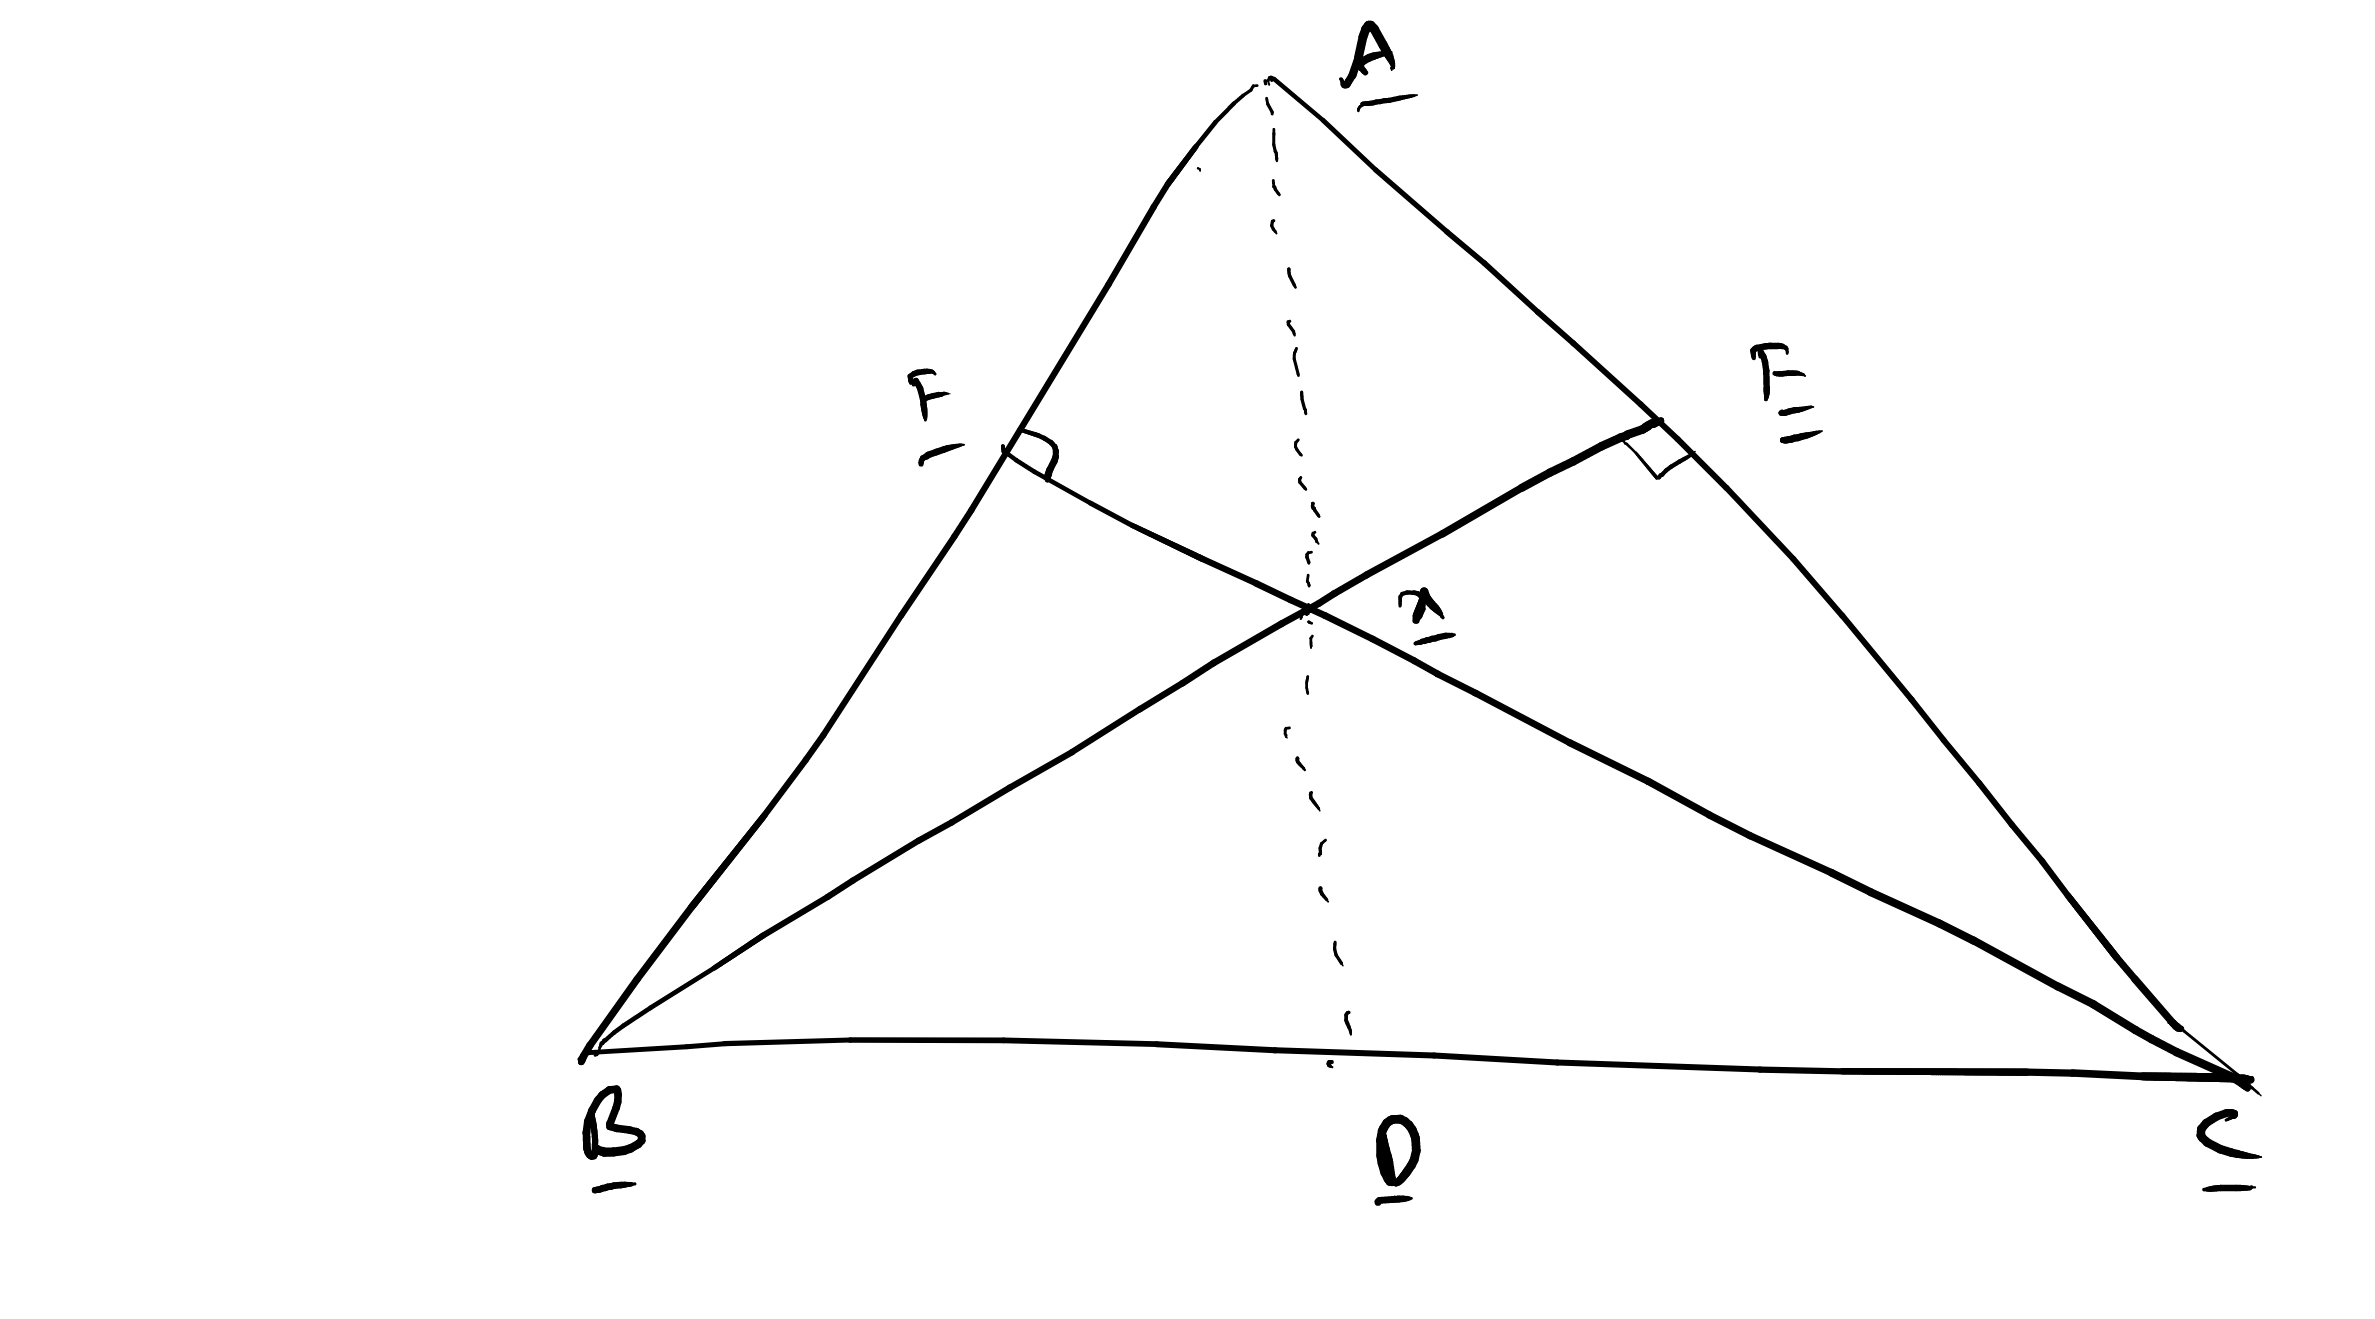
\includegraphics[width=\columnwidth]{./figs/alt.eps}
\caption{}
\label{fig:alt}
\end{figure}
 Let $\vec{x}$ be the intersection of $BE$ and $CF$. Then, using 
\eqref{eq:orth_any},
\begin{align}
\label{eq:alt_1}
\begin{split}
\brak{\vec{x}-\vec{B}}^T
\brak{\vec{A}-\vec{C}} &= 0
\\
\brak{\vec{x}-\vec{C}}^T
\brak{\vec{A}-\vec{B}} &=0
\end{split}
\\
\label{eq:alt_3}
\implies \vec{x}^T\brak{\vec{A}-\vec{C}}-\vec{B}^T\brak{\vec{A}-\vec{C}} &= 0
\\
\text{and }\vec{x}^T\brak{\vec{A}-\vec{B}}-\vec{C}^T\brak{\vec{A}-\vec{B}} &= 0
\label{eq:alt_4}
\end{align}
%
Subtracting \eqref{eq:alt_4} from \eqref{eq:alt_3},
\begin{align}
\vec{x}^T\brak{\vec{B}-\vec{C}} + \vec{A}^T\brak{\vec{C}-\vec{B}} &= 0
\\
\implies \brak{\vec{x}^T - \vec{A}^T}\brak{\vec{B}-\vec{C}}  &= 0
\\
\implies \brak{\vec{x} - \vec{A}}^T\brak{\vec{B}-\vec{C}}  &= 0
\end{align}
%
which completes the proof.
\renewcommand{\theequation}{\theenumi}

\item The line
\begin{align}
\myvec{2 &-8}\vec{x}-4=0
\end{align}
is the perpendicular bisector of the line $AB$ and $\vec{A}$ is the point $\myvec{5\\6}$. What are the coordinates of $\vec{B}$?
\end{enumerate}
